
\chapter{Descriptors}

\section{Definitions and Principles:}

\subsection{Global and Local Features}
In image processing and computer vision tasks, we need to represent the image by
features extracted therefrom. The raw image is perfect for the human eye to extract
all information from; however that is not the case with computer algorithms. There
are generally two methods to represent images, namely, global features and local
features. In the global feature representation, the image is represented by one multidimensional
feature vector, describing the information in the whole image.\\
In other words, the global representation method produces a single vector with values that
measure various aspects of the image such as color, texture or shape. Practically, a
single vector from each image is extracted and then two images can be compared by
comparing their feature vectors.\\ For example, when one wants to distinguish images
of a sea (blue) and a forest (green), a global descriptor of color would produce quite
different vectors for each category. In this context, global features can be interpreted
as a particular property of image involving all pixels.
This property can be color
histograms, texture, edges or even a specific descriptor extracted from some filters
applied to the image \cite{h}.\\ On the other hand, the main goal of local feature representation
is to distinctively represent the image based on some salient regions while
remaining invariant to viewpoint and illumination changes. Thus, the image is represented
based on its local structures by a set of local feature descriptors extracted
from a set of image regions called interest regions (i.e., keypoints) as illustrated in
Fig.\ref{fig:Ft1} Most local features represent texture within the image patch.

\begin{figure}[H]
\centering
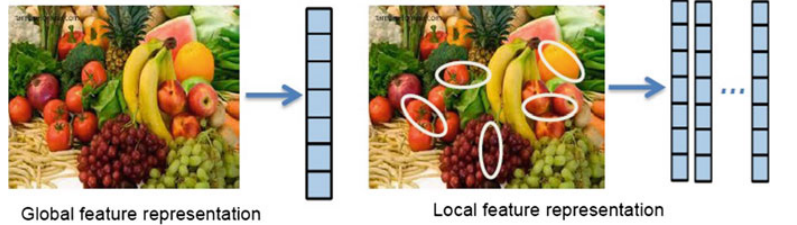
\includegraphics[width=0.9\textwidth]{img/features.PNG}
\caption{ Global and local image features representation }
\label{fig:Ft1}
\end{figure}

Generally, using what kind of features might greatly depend on the applications
on hand. Developers prefer the most discriminative ones. For example, a person with
a bigger nose and smaller eyes, and a person with a smaller nose and bigger eyes
may have similar mug shot in terms of histogram or intensity distribution. Then, local
features or the global pattern distilled from local feature clusters seem to be more
discriminative. Whereas, for very large datasets in the web-scale image indexing
application, it is appropriate to consider global features. Also, global features are
useful in applications where a rough segmentation of the object of interest is available.
The advantages of global features are that they are much faster and compact
while easy to compute and generally require small amounts of memory.\\ Nevertheless,
the global representation suffers from well-known limitations, in particular they
are not invariant to significant transformations and sensitive to clutter and occlusion.\\In some applications, such as copy detection, most of the illegal copies are very
similar to the original; they have only suffered from compression, scaling or limited
cropping. In contrast, the advantage of local features is their superior performance
\cite{i}. Meanwhile, using local features for large-scale image search have much higher
performance than global features provide \cite{k}.\\ Besides, as the local structures are
more distinctive and stable than other structures in smooth regions, it is expected
to be more useful for image matching and object recognition.\\ However, they usually
require a significant amount of memory because the image may have hundreds
of local features.\\ As a solution for this problem, researchers suggest aggregating
local image descriptors into a very compact vector representation and optimizing the
dimensionality reduction of these vectors \cite{k}

\subsection{Characteristics of Feature Detectors}
Tuytelaars and Mikolajczyk \cite{MM} define a local feature as “it is an image pattern
which differs from its immediate neighborhood”. Thus, they consider the purpose of
local invariant features is to provide a representation that allows to efficiently match
local structures between images. That is, we want to obtain a sparse set of local
measurements that capture the essence of the underlying input images and encode
their interesting structures. To meet this goal, the feature detectors and extractors
must have certain properties keeping in mind that the importance of these properties
depends on the actual application settings and compromises need to be made. The
following properties are important for utilizing a feature detector in computer vision
applications:
\begin{itemize}
\item Robustness, the feature detection algorithm should be able to detect the same feature
locations independent of scaling, rotation, shifting, photometric deformations,
compression artifacts, and noise
\item Repeatability, the feature detection algorithm should be able to detect the same
features of the same scene or object repeatedly under variety of viewing conditions.
\item Accuracy, the feature detection algorithm should accurately localize the image
features (same pixel locations), especially for image matching tasks, where precise
correspondences are needed to estimate the epipolar geometry.
\item Generality, the feature detection algorithm should be able to detect features that
can be used in different applications.
\item Efficiency, the feature detection algorithm should be able to detect features in new
images quickly to support real-time applications.
\item Quantity, the feature detection algorithm should be able to detect all or most of the
features in the image. Where, the density of detected features should reflect the
information content of the image for providing a compact image representation.
\end{itemize}

\textbf{in this project We are going to use Local Features( descriptors) For its Efficiency and scale , Rotation  Invariant }\\
\section{Spectra descriptors :}
\subsection{SIFT - Scale Invariant Feature Transforms} \label{siftSection}

Image matching is a fundamental aspect of many problems in computer vision, including
object recognition, solving for 3D structure from multiple images, stereo matching, and
motion tracking and segmentation.\\ This paper describes image features that have many
properties that make them suitable for matching differing images of an object or scene.\\
The features are invariant to image scaling and rotation, and partially invariant to change
in illumination and 3D camera viewpoint. They are well localized in both the spatial and
frequency domains, reducing the probability of disruption by occlusion, clutter, or noise.
Large numbers of features can be extracted from typical images with efficient algorithms.
Most importantly, the features are highly distinctive, which allows a single feature to be
correctly matched with high probability against a large database of features, providing a
basis for object and scene recognition.\\
The cost of extracting these features is minimized by taking a sequential filtering approach,
in which the more expensive operations are applied only at locations that pass an
initial test. Following are the major stages of computation in generating the set of image
features:


\begin{enumerate}
\item Scale-Space Extrema Detection :
The first stage of computation must search over all
scales and image locations, but it can be implemented efficiently by using a difference of-Gaussian
function to identify potential interest points that are invariant to scale and
orientation.
\item Keypoint localization :
At each candidate location, a detailed model is fit to determine
location, scale, and contrast. Keypoints are selected based on measures of their
stability.
\item Orientation assignment :
One or more orientations are assigned to each keypoint
location based on local image properties. All future operations are performed relative
to the assigned orientation, scale, and location for each feature, providing invariance
to these transformations.
\item Keypoint descriptor  :
The local image gradients are measured at the selected scale
in the region around each keypoint, and transformed into a representation that allows
for local shape distortion and change in illumination.
\end{enumerate}

An important aspect of this approach is that it generates large numbers of features that
densely cover the image over the full range of scales and locations.\\ A typical image of size
500$\times$500 pixels will give rise to about 2000 stable features (although this number depends
on both image content and choices for various parameters).\\ The quantity of features is
particularly important for object recognition, where the ability to detect small objects in
cluttered backgrounds requires that at least 3 to 6 features be correctly matched from each
object for reliable identification.
For image matching and recognition, features are first extracted from a set of reference
images and stored in a database.\\ A new image is matched by individually comparing
each feature from the new image to this previous database and finding candidate matching
features based on Euclidean distance of their feature vectors.\\
The keypoint descriptors are highly distinctive, which allows a single feature to find its
correct match with good probability in a large database of features.
\subsection{Scale-Space Extrema Detection :}
As described in [\ref{siftSection}], we will detect keypoints using a sequential filtering approach
that uses efficient algorithms to identify candidate locations that are then examined
in further detail.\\ The first stage of keypoint detection is to identify locations and scales that
can be repeatably assigned under differing views of the same object. Detecting locations
that are invariant to scale change of the image requires that we search for stable features
across all possible changes of scale, using a continuous function of scale known as scale
space (Witkin, 1983).\\
It has been shown by Koenderink (1984) and Lindeberg (1994) that under a variety of reasonable assumptions the only possible scale-space kernel is the Gaussian function.
Therefore, the scale space of an image is defined as a function, L(x, y, $\sigma$), that is produced
from the convolution of a variable-scale Gaussian, G(x, y,$\sigma$), with an input image, I(x, y):\\

L(x, y, $\sigma$) = G(x, y,$\sigma$) * I(x, y),


where * is the convolution operation in x and y, and

\begin{align*} 
 G(x, y,\sigma )  =\frac{1}{2\pi\sigma^2} e^\frac{-( x^2 -  y^2)}{2\sigma^2}  
\end{align*}

To efficiently detect stable keypoint locations in scale space, we have proposed (Lowe,
1999) using scale-space peaks in the difference-of-Gaussian function convolved with the
image, D(x, y, $\sigma$), which can be computed from the difference of two nearby scales separated
by a constant factor k:
\begin{align}
D(x, y, \sigma) &= (G(x, y, k\sigma) - G(x, y,\sigma) * I(x, y)\\
                 &= L(x, y, k\sigma) - L(x, y, \sigma) .
   \end{align}               
                  
There are a number of reasons for choosing this function. First, it is a particularly
efficient function to compute, as the smoothed images, L  need to be computed in any
case for scale space feature description, and D can therefore be computed by simple image
subtraction.

\begin{figure}[H]
\centering
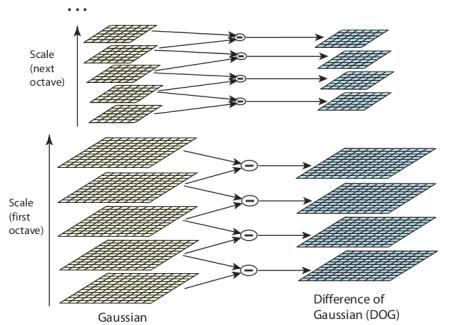
\includegraphics[width=1.0\textwidth]{img/sift_dog.jpg}
\caption{ For each octave of scale space, the initial image is repeatedly convolved with Gaussians to
produce the set of scale space images shown on the left. Adjacent Gaussian images are subtracted
to produce the difference-of-Gaussian images on the right. After each octave, the Gaussian image
is down-sampled by a factor of 2, and the process repeated.}
\label{fig:sift1}
\end{figure}

In addition, the difference-of-Gaussian function provides a close approximation to the
scale-normalized Laplacian of Gaussian, $\sigma^2\nabla^2 G $
, as studied by Lindeberg (1994).\\Lindeberg
showed that the normalization of the Laplacian with the factor $\sigma^2$
is required for true scale invariance. In detailed experimental comparisons, Mikolajczyk (2002) found that the maxima and minima of $\sigma^2\nabla^2 G $  produce the most stable image features compared to a range
of other possible image functions, such as the gradient, Hessian, or Harris corner function.\\
The relationship between D and $\sigma^2\nabla^2G $
G can be understood from the heat diffusion
equation (parameterized in terms of $\sigma$ rather than the more usual t = $\sigma^2$):\\

\begin{align}
    \frac {\partial G} {\partial \sigma} = \sigma \nabla^2 G 
\end{align}




From this, we see that$\nabla^2$ G can be computed from the finite difference approximation to  $\frac{\partial G}{\partial \sigma }$ , using the difference of nearby scales at k$\sigma$ and $\sigma$ :\\


\begin{align}
      \sigma \nabla^2 G =   \frac {\partial G} {\partial \sigma} \approx   \frac {G(x,y,k \sigma) -  G(x,y,\sigma)}{ k \sigma - \sigma}  
\end{align}


and therefore,


\begin{align}
      G(x,y,k \sigma) -  G(x,y,\sigma)  \approx (k - 1)  \sigma^2\nabla^2G 
\end{align}

\begin{figure}[H]
\centering
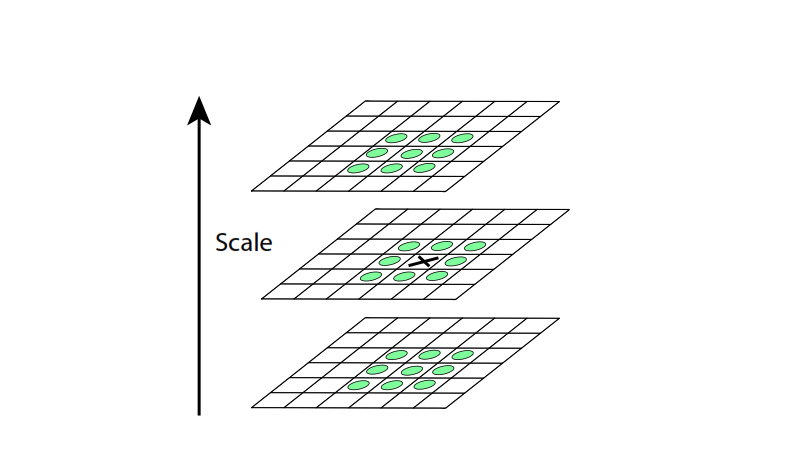
\includegraphics[width=1.0\textwidth]{img/sift2.PNG}
\caption{ Maxima and minima of the difference-of-Gaussian images are detected by comparing a
pixel (marked with X) to its 26 neighbors in 3x3 regions at the current and adjacent scales (marked
with circles).}
\label{fig:sift2}
\end{figure}

This shows that when the difference-of-Gaussian function has scales differing by a constant
factor it already incorporates the  $\sigma ^2 $
scale normalization required for the Laplacian. \\The
factor (k-1) in the equation is a constant over all scales and therefore does not influence
peak location. The approximation error will go to zero as k goes 1, but in practice we have
found that the approximation has almost no impact on the stability of peak detection or
localization for even significant differences in scale, such as $k= \sqrt{2}$
An efficient approach to construction of D(x; y;$\sigma$) is shown in Figure \ref{fig:sift1}. The input image
is incrementally convolved with Gaussians to produce images separated by a constant
factor k in scale space, shown stacked in the left column. \\We choose to divide each octave
of scale space (i.e., doubling of $\sigma$) into an integer number, s, of intervals, so $k = 2^{1/\mathbf{s}}$
Adjacent image scales are subtracted to produce the difference-of-Gaussian images shown
on the right. Once a complete octave has been processed, we resample the Gaussian image
that has twice the initial value of $\sigma$ by taking every second pixel in each row and column. \newline
\newline
The accuracy of sampling relative to $\sigma$ is no different than for the previous octave, while
computation is greatly reduced.

\subsection{Keypoint localization :}
We wish to identify locations in image scale space that are
invariant with respect to image translation, scaling, and rotation,
and are minimally affected by noise and small distortions.\\
Lindeberg \cite{e} has shown that under some rather
general assumptions on scale invariance, the Gaussian kernel
and its derivatives are the only possible smoothing kernels
for scale space analysis.\\
To achieve rotation invariance and a high level of efficiency,
we have chosen to select key locations at maxima
and minima of a difference of Gaussian function applied in
scale space. This can be computed very efficiently by building
an image pyramid with resampling between each level.
Furthermore, it locates key points at regions and scales of
high variation, making these locations particularly stable for
characterizing the image.\\ Crowley and Parker \cite{f} and Lindeberg
\cite{e} have previously used the difference-of-Gaussian in
scale space for other purposes. In the following, we describe
a particularly efficient and stable method to detect and characterize
the maxima and minima of this function.\\
As the 2D Gaussian function is separable, its convolution
with the input image can be efficiently computed by applying
two passes of the 1D Gaussian function in the horizontal
and vertical directions:

\begin{align}
     g(x)  =\frac{1}{\sqrt{2\pi}\sigma} e^\frac{-x^2}{2\sigma^2}
\end{align}


For key localization, all smoothing operations are done using
$\sigma = \sqrt{2}$ , which can be approximated with sufficient accuracy
using a 1D kernel with 7 sample points.\\
The input image is first convolved with the Gaussian
function using $\sigma = \sqrt{2}$ to give an image \textit{A}. This is then
repeated a second time with a further incremental smoothing
of $\sigma = \sqrt{2}$ to give a new image, \textit{B}, which now has an
effective smoothing of $\sigma$ =2. The difference of Gaussian
function is obtained by subtracting image B from A, resulting
in a ratio of $2/\sqrt{2}$ = $ \sqrt{2}$ between the two Gaussians.\\
To generate the next pyramid level, we resample the already smoothed image B using bilinear interpolation with a
pixel spacing of 1.5 in each direction.\\ While it may seem
more natural to resample with a relative scale of$\sqrt{2}$,the
only constraint is that sampling be frequent enough to detect
peaks.\\ The 1.5 spacing means that each newsample will
be a constant linear combination of 4 adjacent pixels. This
is efficient to compute and minimizes aliasing artifacts that
would arise from changing the resampling coefficients.\\
Maxima and minima of this scale-space function are determined
by comparing each pixel in the pyramid to its
neighbours. First, a pixel is compared to its 8 neighbours at
the same level of the pyramid.\\ If it is a maxima or minima
at this level, then the closest pixel location is calculated at
the next lowest level of the pyramid, taking account of the
1.5 times resampling. If the pixel remains higher (or lower)
than this closest pixel and its 8 neighbours, then the test is
repeated for the level above. Since most pixels will be eliminated
within a few comparisons, the cost of this detection is
small and much lower than that of building the pyramid.\\
If the first level of the pyramid is sampled at the same rate
as the input image, the highest spatial frequencies will be ignored.
This is due to the initial smoothing, which is needed
to provide separation of peaks for robust detection. Therefore,
we expand the input image by a factor of 2, using bilinear
interpolation, prior to building the pyramid. This gives
on the order of 1000 key points for a typical
512$\times$512 pixel
image, compared to only a quarter as many without the initial
expansion.
\subsection{Orientation assignment :}
By assigning a consistent orientation to each keypoint based on local image properties,
the keypoint descriptor can be represented relative to this orientation and therefore achieve
invariance to image rotation.\\ This approach contrasts with the orientation invariant descriptors
of Schmid and Mohr (1997), in which each image property is based on a rotationally
invariant measure.\\ The disadvantage of that approach is that it limits the descriptors that
can be used and discards image information by not requiring all measures to be based on a
consistent rotation.\\

Following experimentation with a number of approaches to assigning a local orientation,
the following approach was found to give the most stable results. The scale of the
keypoint is used to select the Gaussian smoothed image, L, with the closest scale, as all
computations must be performed in a scale-invariant manner. For each image sample, $L_{x,y}$ ,the gradient magnitude, m, and orientation, $\theta$, is precomputed using pixel differences:

\begin{align}
 m  =\sqrt{(L_{x+1,y} - L_{x-1,y})^2 + (L_{x,y+1} - L_{x,y-1})^2}
\end{align}
\begin{align}
  \theta = \tan^{\small{-1}}\frac{(L_{x,y+1} - L_{x,y-1})}{(L_{x+1,y} - L_{x-1,y})}
\end{align}

An orientation histogram is formed from the gradient orientations at all sample points
within a circular window around the keypoint. Each sample added to the histogram is
weighted by its gradient magnitude and by a Gaussian-weighted circular window with a $\sigma$
three times that of the scale of the keypoint. The orientation histogram has 36 bins covering
the 360 degree range of orientations.
Peaks in the orientation histogram correspond to dominant directions of local gradients.
The highest local peak in the histogram is detected, and then any other local peak that is
within 80\% of the highest peak is used to also create a keypoint with that orientation.
Therefore, for locations with multiple peaks of similar magnitude, there will be multiple
keypoints created at the same location and scale but different orientations. Only about
15\% of points are assigned multiple orientations, but these contribute significantly to the
stability of matching. Finally, a parabola is fit to the 3 histogram values around each peak
to interpolate the peak position for better accuracy.

\begin{figure}[H]
\centering
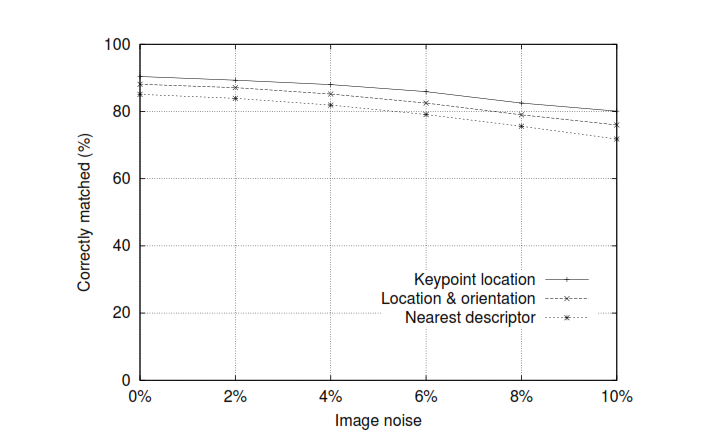
\includegraphics[width=0.7\textwidth]{img/sift3.PNG}
\caption{ The top line in the graph shows the percent of keypoint locations that are repeatably
detected as a function of pixel noise. The second line shows the repeatability after also requiring
agreement in orientation. The bottom line shows the final percent of descriptors correctly matched
to a large database.}
\label{fig:sift3}
\end{figure}

Figure \ref{fig:sift3} shows the experimental stability of orientation assignment under differing
amounts of image noise. As before the images are rotated and scaled by random amounts.
The top line shows the stability of keypoint location. The second line shows the stability of
matching when the orientation assignment is required to be within 15 degrees. As shown
by the gap between the top two lines, the orientation assignment remains accurate 95\% of
the time even after addition of$ \pm$10\% pixel noise (equivalent to truncating pixel values to
less than 3 bits of precision). The measured variance of orientation for the correct matches
is about 2.5 degrees, rising to 3.9 degrees for 10\% noise. The bottom line in Figure \ref{fig:sift3}
shows the final accuracy of correctly matching a keypoint to a large database, which will
be discussed below.

\subsection{Keypoint descriptor :}

Figure \ref{fig:sift4} illustrates the computation of the keypoint descriptor. First the image gradient
magnitudes and orientations are sampled around a keypoint, using the scale of the keypoint
to select the level of Gaussian blur for the image. For efficiency, the gradients are precomputed
for all levels of the pyramid as described in Section 4.1.3 . These are illustrated with
small arrows at each sample location on the left side of Figure \ref{fig:sift4}

\begin{figure}[H]
\centering
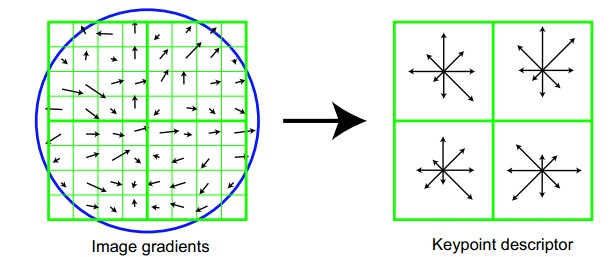
\includegraphics[width=0.8\textwidth]{img/sift4.jpg}
\caption{ A keypoint descriptor is created by first computing the gradient magnitude and orientation
at each image sample point, as shown on the left. These are weighted by a Gaussian window,
indicated by the overlayed circle. These samples are then accumulated into orientation histograms
summarizing the contents over larger regions, as shown on the right, with the length of each arrow
corresponding to the sum of the gradient magnitudes near that direction within the region. To reduce
clutter, this figure shows a 2$\times$2 descriptor array computed from an 8$\times$8 set of samples, whereas most
experiments in this paper use 4x4 descriptors computed from a 16$\times$16 sample array..}
\label{fig:sift4}
\end{figure}

A Gaussian weighting function with $\sigma$ equal to one half the width of the descriptor
window is used to assign a weight to the magnitude of each sample point. This is illustrated
with a circular window on the left side of Figure \ref{fig:sift4}, although, of course, the weight falls off smoothly. The purpose of this Gaussian window is to avoid sudden changes in the
descriptor with small changes in the position of the window, and to give less emphasis
to gradients that are far from the center of the descriptor, as these are most affected by
misregistration errors.
The keypoint descriptor is shown on the right side of Figure \ref{fig:sift4}. It allows for significant
shift in gradient positions by creating orientation histograms over 4$\times$4 sample regions. The
figure shows eight directions for each orientation histogram, with the length of each arrow
corresponding to the magnitude of that histogram entry. A gradient sample on the left can
shift up to 4 sample positions while still contributing to the same histogram on the right,
thereby achieving the objective of allowing for wider local positional shifts.
It is important to avoid all boundary affects in which the descriptor abruptly changes as
a sample shifts smoothly from being within one histogram to another or from one orientation
to another. Therefore, linear interpolation is used to assign a weight to each histogram
entry according to the distance of the sample from its central value, and the gradient magnitude
of a sample is distributed into the histogram accumulators according to these weights.
The descriptor is formed from a vector containing the values of all the orientation histogram
entries, corresponding to the lengths of the arrows on the right side of Figure \ref{fig:sift4}. The
figure shows a 2$\times$2 array of orientation histograms, whereas our experiments below show
that best results are achieved with a 4$\times$4 array of histograms with 8 orientation bins in each.
Therefore, the experiments in this paper use a 4$\times$4$\times$8 = 128 element feature vector for each
keypoint.
Finally, the feature vector is normalized to reduce the effects of illumination change.
First, the vector is normalized to unit length. A change in image contrast in which each
pixel value is multiplied by a constant will multiply gradients by the same constant, so this
contrast change will be cancelled by vector normalization. A brightness change in which a
constant is added to each image pixel will not affect the gradient values, as they are computed
from pixel differences. However, non-linear illumination changes can also occur due
to camera saturation or illumination changes that affect surfaces with different orientations
by differing amounts. These effects can cause a large change in relative magnitudes for
some gradients, but are less likely to affect the gradient orientations. Therefore, we reduce
the influence of gradient magnitudes by thresholding the values in the unit feature vector to
each be no larger than 0.2, and then renormalizing to unit length. This means that matching
the magnitudes for large gradients is no longer as important, and that the distribution of
orientations has greater emphasis. The value of 0.2 was determined experimentally using
differing illuminations for the same objects

\subsection{Speeded Up Robust Features (SURF) :}
SURF (Speeded Up Robust Features), is a feature detector, we talked about SIFT before, and SURF is sort of derivative of SIFT. SURF is based on sums of 2D Haar wavelet responses and makes an efficient use of integral images.

we will not go through  the whole literature  of SURF, because its idea is very similar to SIFT, so we will only talk about \textbf{the difference between these two methods}.

\subsection{ABOUT HESSIAN}
In Sift method, we use Difference of Gaussian (DoG) to build the image pyramid, and in Surf, we simply use an integer approximation to the determinant of Hessian blob detector .

Given a pixel, the Hessian of this pixel is something like:
$\sigma^2\nabla^2G$ \\

\begin{gather}
H(f(x,y)) =
\begin{bmatrix}
                 {\frac {\partial^2 f} {\partial x^2}} && { \frac {\partial^2 f} {\partial x.\partial y} }\\
                 {\frac  {\partial^2 f}{\partial x.\partial y}} && { \frac {\partial^2 f} {\partial y^2}}
\end{bmatrix}
\end{gather}

For adapt to any scale, we filtered the image by a Gaussian kernel, so given a point X = (x, y), the Hessian matrix H(x,$\sigma$) in x at scale σ is defined as:
\begin{gather}
 \mathcal{H}(x,\sigma) =
\begin{bmatrix}
                 {L_{xx}(x,\sigma)}  && {L_{xy}(x,\sigma)} \\
                 {L_{xy}(x,\sigma)} && {L_{yy}(x,\sigma)}
\end{bmatrix}
\end{gather}
where ${L_{xx}(x,\sigma)}$ is the convolution of the Gaussian second order derivative with the image I in point x, and similarly for ${L_{xy}(x,\sigma)}$ and ${L_{yy}(x,\sigma)}$.\\
First convolution, then second order derivative, we now approximate these two processes with one single filter.\\


\begin{figure}[H]
\centering
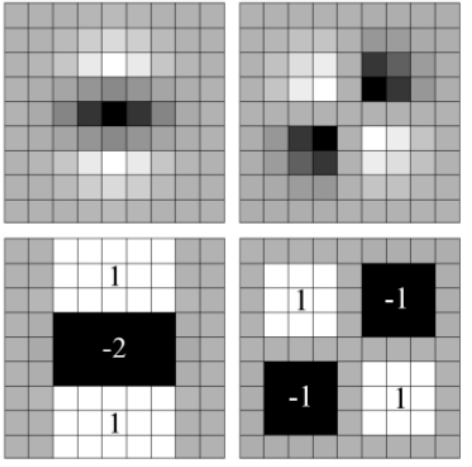
\includegraphics[width=0.55\textwidth]{img/surf4.PNG}
\caption{${L_{yy}(x,\sigma)}$ and${L_{xy}(x,\sigma)}$ Discretized
Gaussians and the approximations $D_{yy}$ and $D_{xy}$}
\label{fig:surf1}
\end{figure}

These approximate second order Gaussian derivatives and can be evaluated at a very low computational cost using integral images, and this is part of the reason why SURF is fast.

Now we can represent the determinant of the Hessian (approximated) as:



\subsection{ABOUT PYRAMID :}

In Sift, we use DOG to build image pyramids, the pyramid have several octaves, and there are several images layers in each octave. The difference between Sift pyramid and Surf pyramid is, in Sift, we use different scales of image; and in Surf, we use different scales of Gaussian masks, while the scale of image is always unaltered. By this, we save a lot of time by not downsampling image.

\begin{figure}[H]
\centering
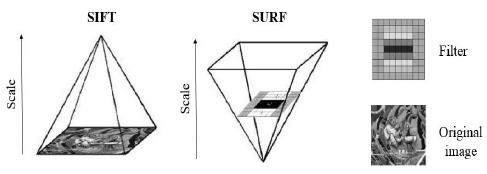
\includegraphics[width=0.6\textwidth]{img/surf2.png}
\caption{Where SIFT(left) downscales the image,
SURF(right) uses larger and larger filters}
\label{fig:surf2}
\end{figure}

 Instead of iteratively reducing the image size (left), the use of integral images allows the up-scaling of the filter at constant cost (right).\\
 
 \subsection{ABOUT FEATURE DESCRIPTOR}
 In Sift, we use an orientation histogram, and find the largest orientation value and also those values that are over 80\% of the largest, and use these orientations as the main orientation of the feature descriptor. In Surf, we use the sum of the Haar wavelet response around the point of interest.

\begin{figure}[H]
\centering
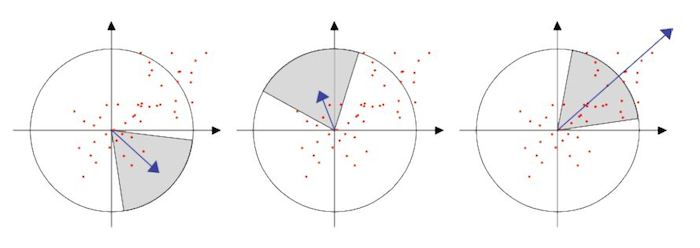
\includegraphics[width=0.6\textwidth]{img/surf3.jpg}
\caption{descriptor computation }
\label{fig:surf2}
\end{figure}

We first calculate the Haar wavelet responses in x and y direction within a circular neighborhood of radius 6s around the interest point, with s the scale at which the interest point was detected. We calculate the sum of vertical and horizontal wavelet responses in a scanning aria, then change the scanning orientation (add $\pi$/3), and re-calculate, until we find the orientation with largest sum value, this orientation is the main orientation of feature descriptor.

Now it’s time to extract the descriptor. First we construct a square region centered around the feature point, and oriented along the main orientation we already got above, the size of this window is 20s,s is the scale at which the interest point was detected. Second we split this region up regularly into smaller 4$\times$4 square subregions, for each sub-region, we compute Haar wavelet responses at 5$\times$5 regularly spaced sample points.


\begin{figure}[H]
\centering
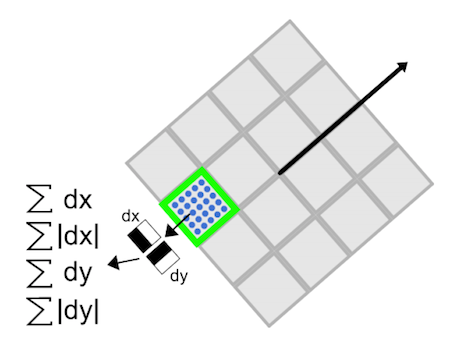
\includegraphics[width=0.6\textwidth]{img/surf5.png}
\caption{computation of dx and dy of Haar  }
\label{fig:surf5}
\end{figure}

We extract the sum of values of the responses in both x and y orientation, furthermore, we extract the sum of the absolute values of the responses, hence, each sub-region has a 4-D descriptor vector v. Concatenating this for all 4$\times$4 sub-regions, our final descriptor is a 64-D vector. (In Sift, our descriptor is 128-D vector, so this is part of the reason that SURF is faster than Sift.)


\subsection{Histogram of Gradients (HOG) Descriptor  and its Variants :}

The Histogram of Gradients (HOG) method \cite{g} is intended for image classification,
and relies on computing local region gradients over a dense grid of overlapping blocks,
rather than at interest points. HOG is appropriate for some applications, such as person
detection, where the feature in the image is quite large.
HOG operates on raw data; while many methods rely on Gaussian smoothing and
other filtering methods to prepare the data, HOG is designed specifically to use all the
raw data without introducing filtering artifacts that remove fine details. The authors show
clear benefits using this approach. It’s a tradeoff: \textit{filtering artifacts} such as smoothing vs.
image artifacts such as fine details. The HOG method shows preferential results for the
raw data. See Figure 4-12, showing a visualization of a HOG descriptor.
Major aspects in the HOG method are as follows:

\begin{itemize}
\item Raw RGB image is used with no color correction or noise filtering,
using other color spaces and color gamma adjustment provided
little advantage for the added cost
\item Prefers a 64x128 sliding detector window; 56x120 and 48x112
sized windows were also tested. Within this detector window, a
total of 8x16 8x8 pixel block regions are defined for computation
of gradients. Block sizes are tunable.
\item For each 8x8 pixel block, a total of 64 local gradient magnitudes
are computed. The preferred method is simple line and column
derivatives [-1,0,1] in x/y; other gradient filter methods are tried,
but larger filters with or without Gaussian filtering degrade
accuracy and performance. Separate gradients are calculated for
each color channel
\item Local gradient magnitudes are binned into a 9-bin histogram of
edge orientations, quantizing dimensionality from 64 to 9, using
bilinear interpolation; $<$9 bins produce poorer accuracy, $>$9 bins
does not seem to matter. Note that either rectangular R-HOG or
circular log polar C-HOG binning regions can be used.
\item Normalization of gradient magnitude histogram values to
unit length to provide illumination invariance. Normalization
is performed in groups, rather than on single histograms.
Overlapping 2x2 blocks of histograms are used within the detector
window; the block overlapping method reduces sharp artifacts,
and the 2x2 region size seems to work best.
\item For the 64x128 pixel detector window method, a total of 128
8x8 pixel blocks are defined. Each 8x8 block has four cells for
computing separate 9-bin histograms. The total descriptor size is
then 8x16x4x9=4608.
\end{itemize}
Note that various formulations of the sliding window and block sizes are used for
dealing with specific application domains. See Figure 4-12, showing a visualization of
HOG descriptor computed using 7x15 8x8 pixel cells. Key findings from the HOG \cite{g}
design approach include:
\begin{itemize}
\item The abrupt edges at fine scales in the raw data are required for
accuracy in the gradient calculations, and post-processing and
normalizing the gradient bins later works well
\item L2 style block normalization of local contrast is preferred and
provides better accuracy over global normalization; note that the
local region blocks are overlapped to assist in the normalization.
\item Dropping the L2 block normalization stage during histogram
binning reduces accuracy by 27 percent.
\item HOG features perform much better than HAAR-style detectors,
and this makes sense when we consider that a HAAR wavelet is
an integrated directionless value, while gradient magnitude and
direction over the local HOG region provides a richer spectra.

\end{itemize}

\textbf{HOG Summary Taxonomy}\\
\\
Spectra: Local region gradient histograms\\
Feature shape: Rectangle or circle\\
Feature pattern: Dense  64$\times$128  typical rectangle\\
Feature density: Dense overlapping blocks\\
Search method: Grid over scale space\\
Distance function: Euclidean\\
Robustness: 4 (illumination, viewpoint, scale, noise)


\section{Binary descriptors :}

The SIFT keypoint detector and descriptor,4 although over a decade old, have proven to be remarkably successful
in a number of applications using visual features, including object detection and recognition, image stitching,
scene classification, etc. This descriptor has been also extended to color images in the form of RGB-SIFT,
Opponent-SIFT and C-SIFT, as described by van de Sande et al. in.5 However, it requires an intensive computational
effort, especially for real-time systems, or for low-power devices such as cellphones. This has led to
an increased research for replacements with simpler descriptors with lower computation demands. This trend
started with SURF,6 but since then a lot of other descriptors have been proposed in literature, always focusing
not only on performance but also on speed: we can refer to ORB , BRISK ,BRIEF, FREAK among the most recent
proposals. There has also been research aimed at speeding up the computation of SIFT, most notably with GPU
devices, or the exploitation of approximate nearest neighbor techniques, starting from LSH up to product
quantization.
Also a great variety of global features has been proposed to tackle the retrieval problem, for example color
histograms, GIST and HOG. Usually these features are easier to compute and do not require the quantization
step typical of the bag-of-words model which is necessary to create a global representation (an histogram of visual
words) from the aforementioned local descriptors.

\subsection{The BRISK descriptor}
The BRISK descriptor \cite{AA} point-pair sampling shape is symmetric and circular,
composed of 60 total points arranged in four concentric rings, as shown in Figure \ref{fig:brisk}.
Surrounding each of the 60 points is a sampling region shown in blue, the sampling
regions increase in size with distance from the center, and also proportional to the
distance between sample points. Within the sampling regions, Gaussian smoothing is
applied to the pixels and a local gradient is calculated over the smoothed region.

\begin{figure}[H]
\centering
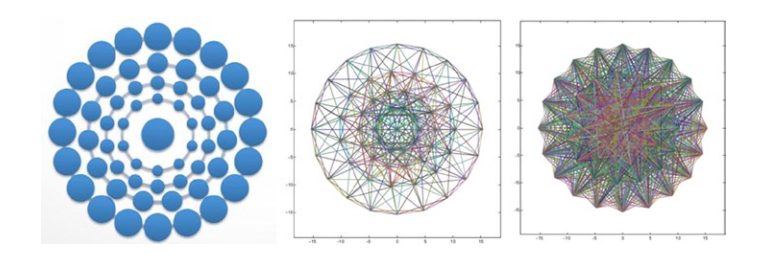
\includegraphics[width=0.8\textwidth]{img/brisk.PNG}
\caption{ (Left) BRISK concentric sampling grid pattern. (Center) Short segment pairs.
(Right) Long distance pairs. Note that the size of the region (left image) for each selected
point increases in diameter with distance from the center, and the binary comparison is
computed from the center point of each Gaussian-sampled circular region, rather than
from each solitary center point. (Center and right images used by permission © Josh
Gleason \cite{AAA}) }
\label{fig:brisk}
\end{figure}


Like other local binary descriptors, BRISK compares pairs of points to form the
descriptor. The point- pairs are specified in two groups: (1) \textbf{long segments}, which are used
together with the region gradients to determine angle and direction of the descriptor,
the angle is used to rotate the descriptor area, and then the pair–wise sampling pattern is
applied;(2) \textbf{short segments}, which can be pair-wise compared and composed into the
512-bit binary descriptor vector.
\subsection{ORB Descriptor }
(Oriented FAST rotated BRISK) is a 
combination of FAST and BRISK. To extract keypoints, it
modifies the FAST detector as scale invariant by constructing a
scale pyramid of the image. At each scale, keypoints are detected
by illustrating the FAST detector. Once the keypoints detected,
the Harris corner measure is employed to sort them and only top
N points are chosen based on a threshold. To obtain rotation
invariant features, first-order moments is used to compute the
local orientation through an intensity centroid which refers to the
weighted averaging of pixel magnitudes in the local patch.
BRIEF descriptors further are computed on rotated patch and
keeps the binary string as ORB descriptor.

\subsection{FREAK }
is also a binary descriptor and borrows the 
procedures of sampling pattern and pair selection from BRISK. 
It uses a circular pattern where the density of points exponentially
drops when moving away from the center and called as retinal
sampling grid that inspired by the retinal pattern in the eye. To
provide rotation invariance property, an orientation for the 
selected patch is computed by summing the local gradients over
chosen pairs which are symmetric to each other with when center
is considered as base. Also, in descriptor creation stage, a similar
approach that was used in ORB is performed, simply the less
correlated pattern is selected. Generally, the 512 binary tests are
used in order to obtain maximum performance. 


\section{Fourier Shape Descriptor } \label{FDT}
The Fourier transformed coefficients from the Fourier
Descriptors of the shape represent the shape of the object in
the frequency domain. The general features of the shape can
be found in the lower frequency descriptors, while the higher
frequency descriptors contain information about the shape
details \cite{20}
Before applying Fourier transform on the shape boundary, it
is first normalized for matching purposes; this is done by
sampling the boundary of each shape to have the same number
of data points. The larger the number of sampled points the
more details in the representation of the shape this results in
more accurate matching. While a smaller number of sampled
points reduce the accuracy of the matching results but on the
other hand it will improve the computational efficiency. \\

After normalization we to apply Fourier transform to the
shape signature. A shape signature is any 1-D function
representing 2-D areas or boundaries. The shape signature we
used is complex coordinates. A complex coordinates function
is the complex form of the boundary coordinates \cite{20}. \\
\begin{gather}
    z_{i} = x_{i}+j y_{i} , i\in [1,N]
\end{gather}\\
For each shape we select N points with equal point
sampling. In order to facilitate the use of Fast Fourier
Transform (FFT), the number of sampled points is chosen to
be power-of-two. Assuming the number of sampled points is
N the Fourier transform gives N Fourier coefficients Cl. The
coefficients are usually called Fourier descriptors of the shape. 
\begin{gather}
C_{l}= \sum_{i=0}^{N-1} z_{i}e{\frac{-j 2\pi il}{N}} , l = 0,...,N-1
\end{gather}
The magnitude of the Fourier
Transform of this set forms a unique shape signature, which can be used for generalized
gesture classification.
In addition, this descriptor is rotationally invariant. Shifts in the silhouette contour
points, which is the cause of rotation, will be appear as phase delays in frequency
domain. However, since only the magnitude of the Fourier coefficients is considered,
the phase (or equivalently, the rotation) is ignored. So, this method is rotationally
invariant while remaining computationally fast\\


\textbf{Generating the Fourier Descriptor: }\\
\begin{enumerate}
    \item $X_{c} = \frac{1}{N}\sum_{n=0}^{N-1} x(i) , Y_{c} = \frac{1}{N}\sum_{n=0}^{N-1} y(i)  = 1$ , where N is number of hand object pixels 
    \item Take the magnitude of the N point DFT of these points :\\
              \textbf{ abs(FT{r[n]}) = a[m] , for m = 0..N-1 }.
    \item Normalize the Fourier coefficients by the DC value (Scale Invariance) .
    \item Keep the first 7 normalized coefficients (skip DC, which is always 1) .

\end{enumerate}


This is the Fourier Descriptor for a single shape.\\
\\
\textbf{Make a Dictionary :}\\
For a set of images of the same gesture, compute the average Fourier shape descriptor
and add it to the dictionary with the same label. Repeat for all desired gestures.\\
\textbf{Classification}\\
Compute the Fourier descriptor for each new sample. Compare it with each stored
gesture in the dictionary using a Euclidean distance measure. The label of the minimum
distance is the desired gesture \\
\textbf{( Nearest Neighbor  happens to be the most efficient method of classification  ) }

\subsection{Covariance Matrix Approach :}
This approach \cite{21}
performs human action recognition by looking at a sequence of whole body silhouettes
over time, a silhouette tunnel, captured by the Kinect. A 13 dimensional feature vector
is defined, where 3 values are row, column, and time, 8 values are based on the shape of
the silhouette, and the last 2 are a measure of the temporal similarity.
However, this feature vector is general enough to work with hand silhouettes in addition
to full bodies. So, it is possible to modify the shape feature vector to work with static
hand gestures by reducing the dimensionality. This can be accomplished by removing
the time dependence and temporal similarity terms. The result is a generalized 10
dimensional feature vector applicable to static shape recognition.\\

\textbf{Create the Feature Vector :}\\
\begin{enumerate}
    \item Compute the 10-dimensional feature vector adapted from Guo \cite{21} : 
    
    \item f(x,y) = [x,y,de,dw,dn,ds,dne,dse,dnw]
    \begin{itemize}
        \item x = col , y=row
        \item d =  Euclidean distance from (x,y) to the nearest boundary point in the specified
direction \\
east, west, north, south, northeast, southwest, southeast, northwest
    \end{itemize}
    \item Scale Invariance 
    \begin{itemize}
        \item Divide each spatial feature by the square root of the silhouette area
     
    \end{itemize}
    \item Compute the Covariance Matrix: 
    \begin{itemize}
        \item $cov(f(\textbf{S}))=\frac{1}{|S|}\sum_{(x,y) \in S }(f(x,y)-\mu_{F})(f(x,y)-\mu_{F})^{T}$
        \item \textbf{S} = area of silhouettte 
        \item $\mu_{F} = \frac{1}{|S|}\sum_{(x,y) \in S } f(x,y) $
    \end{itemize}
    
\end{enumerate}
\textbf{Build a Dictionary }\\
For a set of images of the same gesture, compute the Covariance Matrix and add it to
the dictionary with the same label. Repeat for all desired gestures.\\
\textbf{Classification }\\
As noted in Guo \cite{21}, the set of all covariance matrices lie on a Riemannian
manifold. So, a Euclidean distance measure cannot be used. Instead, the distance
between two covariance matrices on this manifold is defined as:\\
$$d(C,C') = \sqrt{\sum_{k=1}^{10} (\ln \lambda_{k}(C,C'))^{2}}$$ \\
\texttt{where $\lambda_{k}(C,C')$ are generalized eigenvalues of C and C'\\
C = convariance Matrix of new sample ,  C' = Reference from dictionary  } \\

The label of the minimum distance gesture is used for classification .\\
% Please add the following required packages to wer document preamble:
% Please add the following required packages to your document preamble:
% \usepackage{graphicx}
% Please add the following required packages to your document preamble:
% \usepackage{graphicx}
% Please add the following required packages to your document preamble:
% \usepackage{graphicx}
\begin{table}[!h]
\centering
\caption{Pros and Con of Covariance approach }
\label{my-label}
\begin{tabular}{lllll}
\cline{1-2}
\multicolumn{1}{|l|}{\textbf{\begin{tabular}[c]{@{}l@{}}Pros:\\  1. Complex Gesture .\\  2. High accuracy.\\  3. Scale invariant.\end{tabular}}} & \multicolumn{1}{l|}{\textbf{\begin{tabular}[c]{@{}l@{}}Con :\\ 1. Not rotation Invariant . \\           \\        \\ \end{tabular}}} &  &  &  \\ \cline{1-2}
                                                                                                                                                 &                                                                                                           &  &  &  \\
                                                                                                                                                 &                                                                                                           &  &  &  \\
                                                                                                                                                 &                                                                                                           &  &  & 
\end{tabular}
\end{table}\\
\newpage
 \section{ Conclusion : }
 in this chapter we went through Two types of descriptors :\\
\textbf{the first} are  Local descriptors which contains two types \textbf{Spectra descriptors( SIFT and SURF ...) and Binary descriptors( ORB , FREAK ,BRIEF...)} , the spectra group of descriptors typically involves more intense computations and algorithms, often requiring floating point
calculations, and may consume considerable memory. In this taxonomy and discussion,
spectra is simply a quantity that can be measured or computed, such as light intensity,
color, local area gradients, local area statistical features and moments, surface normals,
and sorted data such 2D or 3D histograms of any spectral type, such as histograms of
local gradient direction. Many of the methods discussed in section 4.2 use local gradient
information.\\
Local binary descriptors, as discussed in the previous section, are an attempt
to move away from more costly spectral methods to reduce power and increase
performance. Local binary descriptors in many cases offer similar accuracy and
robustness to the more compute-intensive spectra methods. \\
\textbf{The second } are Basis Space descriptors   , A basis space is composed of a set of functions, the basis functions, which are
composed together as a set, such as a series like the Fourier series and covariance Matrix  . \\
Fourier descriptors represent feature data as sine and cosine terms, which can be
observed in a Fourier Power Spectrum. The Fourier series, Fourier transform, and Fast
Fourier transform are used for a wide range of signal analysis, including 1D, 2D, and 3D
problems. No discussion of image processing or computer vision is complete without
Fourier methods .